This section treats the determination of the emissivity of the paint. To do so, we need the paint to be next to a surface of known emissivity. We use high emissivity tape with $\epsilon_\text{T} = \SI{0.95}{}$. In terms of equation \eqref{eq:powerTemp}, we can then write
\begin{align*}
	P_\text{P} &= \epsilon_\text{P}F(T_\text{P}) + (1-\epsilon_\text{P})F(T_\text{amb}) \ , \\
	P_\text{T} &= \epsilon_\text{T}F(T_\text{T}) + (1-\epsilon_\text{T})F(T_\text{amb}) \ .
\end{align*}
Assuming that both areas have the same real temperature because of their proximity and therefore emit the same amount of IR radiation, we set $P_\text{P}=P_\text{T}$. After rearranging, we obtain an equation for the emissvity of the paint
\begin{align}
	\epsilon_\text{P} = \epsilon_\text{T}\frac{F(T_\text{T})-F(T_\text{amb})}{F(T_\text{P})-F(T_\text{amb})} \ .
\end{align}



In the following, we first describe the used set-up for measuring the emissivity of the paint and afterwards analyse the obtained data.
\subsection{Set-Up}
As the petal will later be used at temperatures below \SI{0}{\degreeCelsius}, also the thermal performance tests need to be adapted to low temperatures. Therefore, we measure the emissivity of the paint on the cold side of a Peltier element. Figure \ref{fig:peltier} shows the used Peltier.
To ensure a low humidity to avoid ice formation, the Peltier sits in a cardboard box with dry air flushing that only leaves a hole for the camera lens.
\begin{figure}[h!]
	\centering
	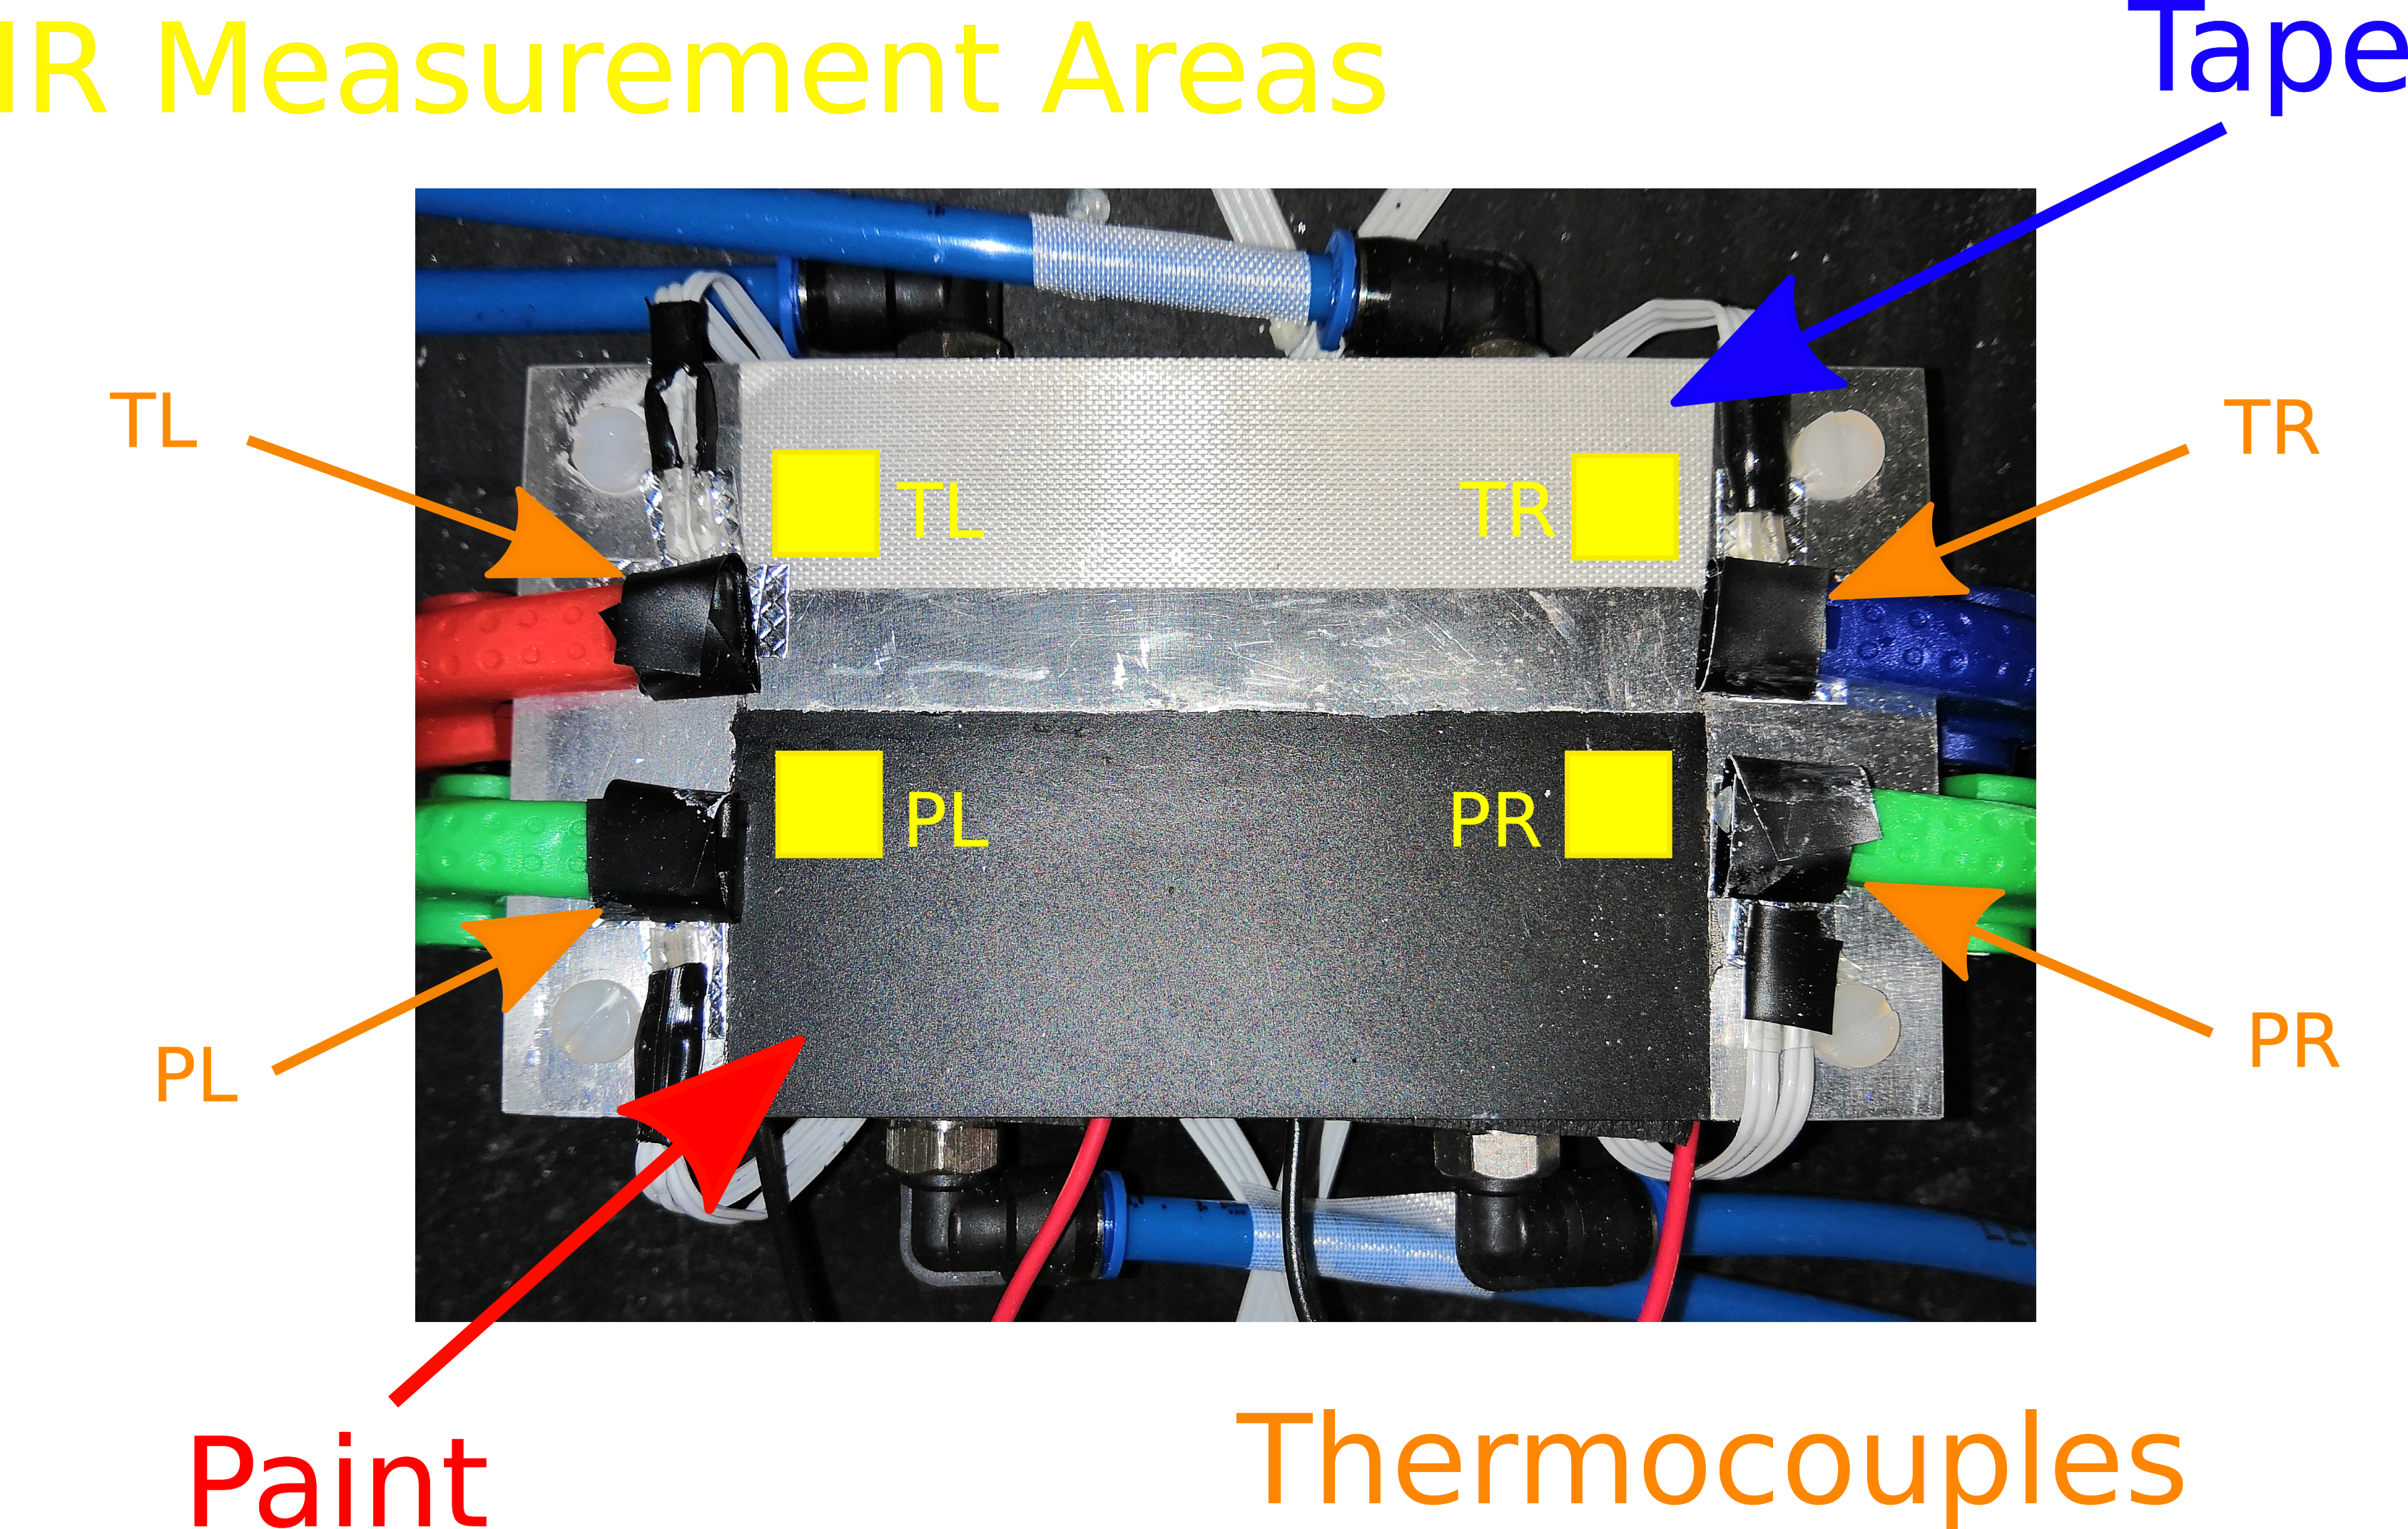
\includegraphics[width=0.8\textwidth]{img/PeltierBeschriftet.png}
	\caption{Peltier element used for measuring the emissivity of the paint. We see the cold side with a taped and a painted area. There are also for thermocouples (type: pt100) which are named according to their position (e.g. TL means tape left). Additionally there is an IR camera measurement area next to each of the thermocouples.}
	\label{fig:peltier}
\end{figure} \\


\subsection{Results}


\clearpage